\documentclass[tikz,border=8pt]{standalone}
% Shared look for every TikZ diagram. Load with \input{../../tools/tikz-style.tex}
\usepackage[T1]{fontenc}
\usepackage{lmodern}
\renewcommand{\sfdefault}{lmr}  % diagrams use the same serif as the text
\usetikzlibrary{arrows.meta, positioning, shapes.geometric, calc, fit, backgrounds}
\definecolor{cblue}{HTML}{4C78A8}
\definecolor{corange}{HTML}{F58518}
\definecolor{cgreen}{HTML}{54A24B}
\definecolor{cred}{HTML}{E45756}
\definecolor{cpurple}{HTML}{B279A2}
\definecolor{cgrey}{HTML}{6B6B6B}
\tikzset{
  every picture/.style={font=\sffamily, line width=1.2pt},
  box/.style={draw=#1, fill=#1!12, rounded corners=4pt, align=center, inner sep=7pt, minimum height=1.1cm},
  box/.default=cgrey,
  arrow/.style={-{Stealth[length=3mm]}, draw=cgrey, line width=1.4pt},
  title/.style={font=\sffamily\bfseries\Large},
  note/.style={font=\sffamily\small, text=cgrey, align=center},
}
\AtBeginDocument{\hyphenpenalty=10000 \exhyphenpenalty=10000}

\begin{document}
% Section 3: Luong's three equations for decoder step 2 ("la"): dot products of s_2 with every encoder state,
% softmax, weighted sum of the encoder states.
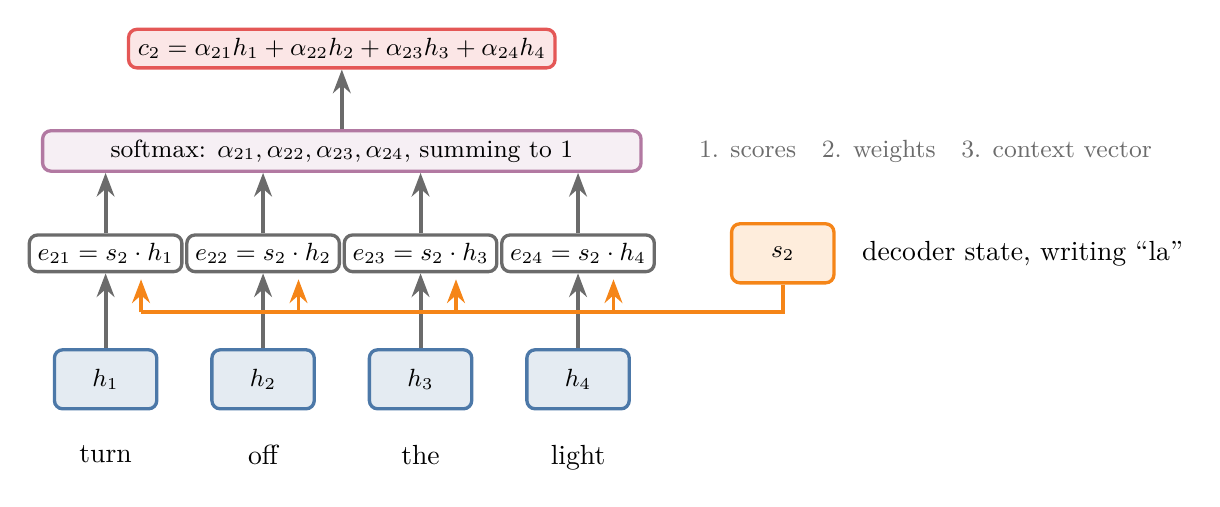
\begin{tikzpicture}[cell/.style={draw=#1, fill=#1!15, minimum width=1.3cm, minimum height=0.75cm, rounded corners=3pt, font=\sffamily\small},
  op/.style={draw=cgrey, fill=white, rounded corners=3pt, font=\sffamily\small, inner sep=3pt}]
  \foreach \w [count=\j] in {turn, off, the, light} {
    \node[cell=cblue] (h\j) at (2.0*\j, 0) {$h_\j$};
    \node[font=\sffamily, below=0.3cm of h\j] {\w};
    \node[op] (e\j) at (2.0*\j, 1.6) {$e_{2\j} = s_2 \cdot h_\j$};
    \draw[arrow] (h\j) -- (e\j);
  }
  \node[cell=corange] (s2) at (10.6, 1.6) {$s_2$};
  \node[font=\sffamily, right=0.2cm of s2] {decoder state, writing ``la''};
  \draw[draw=corange, line width=1.4pt] (s2.south) |- (2.45, 0.85);
  \foreach \j in {1,...,4} \draw[arrow, draw=corange] (2.0*\j + 0.45, 0.85) -- (2.0*\j + 0.45, 1.27);
  \node[draw=cpurple, fill=cpurple!12, rounded corners=3pt, minimum width=7.6cm, font=\sffamily\small] (sm) at (5.0, 2.9)
    {softmax: $\alpha_{21}, \alpha_{22}, \alpha_{23}, \alpha_{24}$, summing to 1};
  \foreach \j in {1,...,4} \draw[arrow] (e\j) -- (e\j |- sm.south);
  \node[draw=cred, fill=cred!15, rounded corners=3pt, font=\sffamily\small] (c) at (5.0, 4.2)
    {$c_2 = \alpha_{21}h_1 + \alpha_{22}h_2 + \alpha_{23}h_3 + \alpha_{24}h_4$};
  \draw[arrow] (sm) -- (c);
  \node[note, anchor=west] at (9.4, 2.9) {1. scores\quad 2. weights\quad 3. context vector};
\end{tikzpicture}
\end{document}
